% Options for packages loaded elsewhere
\PassOptionsToPackage{unicode}{hyperref}
\PassOptionsToPackage{hyphens}{url}
%
\documentclass[
]{article}
\usepackage{lmodern}
\usepackage{amssymb,amsmath}
\usepackage{ifxetex,ifluatex}
\ifnum 0\ifxetex 1\fi\ifluatex 1\fi=0 % if pdftex
  \usepackage[T1]{fontenc}
  \usepackage[utf8]{inputenc}
  \usepackage{textcomp} % provide euro and other symbols
\else % if luatex or xetex
  \usepackage{unicode-math}
  \defaultfontfeatures{Scale=MatchLowercase}
  \defaultfontfeatures[\rmfamily]{Ligatures=TeX,Scale=1}
\fi
% Use upquote if available, for straight quotes in verbatim environments
\IfFileExists{upquote.sty}{\usepackage{upquote}}{}
\IfFileExists{microtype.sty}{% use microtype if available
  \usepackage[]{microtype}
  \UseMicrotypeSet[protrusion]{basicmath} % disable protrusion for tt fonts
}{}
\makeatletter
\@ifundefined{KOMAClassName}{% if non-KOMA class
  \IfFileExists{parskip.sty}{%
    \usepackage{parskip}
  }{% else
    \setlength{\parindent}{0pt}
    \setlength{\parskip}{6pt plus 2pt minus 1pt}}
}{% if KOMA class
  \KOMAoptions{parskip=half}}
\makeatother
\usepackage{xcolor}
\IfFileExists{xurl.sty}{\usepackage{xurl}}{} % add URL line breaks if available
\IfFileExists{bookmark.sty}{\usepackage{bookmark}}{\usepackage{hyperref}}
\hypersetup{
  pdftitle={Oblig 1, Sanders},
  hidelinks,
  pdfcreator={LaTeX via pandoc}}
\urlstyle{same} % disable monospaced font for URLs
\usepackage[margin=1in]{geometry}
\usepackage{color}
\usepackage{fancyvrb}
\newcommand{\VerbBar}{|}
\newcommand{\VERB}{\Verb[commandchars=\\\{\}]}
\DefineVerbatimEnvironment{Highlighting}{Verbatim}{commandchars=\\\{\}}
% Add ',fontsize=\small' for more characters per line
\usepackage{framed}
\definecolor{shadecolor}{RGB}{248,248,248}
\newenvironment{Shaded}{\begin{snugshade}}{\end{snugshade}}
\newcommand{\AlertTok}[1]{\textcolor[rgb]{0.94,0.16,0.16}{#1}}
\newcommand{\AnnotationTok}[1]{\textcolor[rgb]{0.56,0.35,0.01}{\textbf{\textit{#1}}}}
\newcommand{\AttributeTok}[1]{\textcolor[rgb]{0.77,0.63,0.00}{#1}}
\newcommand{\BaseNTok}[1]{\textcolor[rgb]{0.00,0.00,0.81}{#1}}
\newcommand{\BuiltInTok}[1]{#1}
\newcommand{\CharTok}[1]{\textcolor[rgb]{0.31,0.60,0.02}{#1}}
\newcommand{\CommentTok}[1]{\textcolor[rgb]{0.56,0.35,0.01}{\textit{#1}}}
\newcommand{\CommentVarTok}[1]{\textcolor[rgb]{0.56,0.35,0.01}{\textbf{\textit{#1}}}}
\newcommand{\ConstantTok}[1]{\textcolor[rgb]{0.00,0.00,0.00}{#1}}
\newcommand{\ControlFlowTok}[1]{\textcolor[rgb]{0.13,0.29,0.53}{\textbf{#1}}}
\newcommand{\DataTypeTok}[1]{\textcolor[rgb]{0.13,0.29,0.53}{#1}}
\newcommand{\DecValTok}[1]{\textcolor[rgb]{0.00,0.00,0.81}{#1}}
\newcommand{\DocumentationTok}[1]{\textcolor[rgb]{0.56,0.35,0.01}{\textbf{\textit{#1}}}}
\newcommand{\ErrorTok}[1]{\textcolor[rgb]{0.64,0.00,0.00}{\textbf{#1}}}
\newcommand{\ExtensionTok}[1]{#1}
\newcommand{\FloatTok}[1]{\textcolor[rgb]{0.00,0.00,0.81}{#1}}
\newcommand{\FunctionTok}[1]{\textcolor[rgb]{0.00,0.00,0.00}{#1}}
\newcommand{\ImportTok}[1]{#1}
\newcommand{\InformationTok}[1]{\textcolor[rgb]{0.56,0.35,0.01}{\textbf{\textit{#1}}}}
\newcommand{\KeywordTok}[1]{\textcolor[rgb]{0.13,0.29,0.53}{\textbf{#1}}}
\newcommand{\NormalTok}[1]{#1}
\newcommand{\OperatorTok}[1]{\textcolor[rgb]{0.81,0.36,0.00}{\textbf{#1}}}
\newcommand{\OtherTok}[1]{\textcolor[rgb]{0.56,0.35,0.01}{#1}}
\newcommand{\PreprocessorTok}[1]{\textcolor[rgb]{0.56,0.35,0.01}{\textit{#1}}}
\newcommand{\RegionMarkerTok}[1]{#1}
\newcommand{\SpecialCharTok}[1]{\textcolor[rgb]{0.00,0.00,0.00}{#1}}
\newcommand{\SpecialStringTok}[1]{\textcolor[rgb]{0.31,0.60,0.02}{#1}}
\newcommand{\StringTok}[1]{\textcolor[rgb]{0.31,0.60,0.02}{#1}}
\newcommand{\VariableTok}[1]{\textcolor[rgb]{0.00,0.00,0.00}{#1}}
\newcommand{\VerbatimStringTok}[1]{\textcolor[rgb]{0.31,0.60,0.02}{#1}}
\newcommand{\WarningTok}[1]{\textcolor[rgb]{0.56,0.35,0.01}{\textbf{\textit{#1}}}}
\usepackage{graphicx,grffile}
\makeatletter
\def\maxwidth{\ifdim\Gin@nat@width>\linewidth\linewidth\else\Gin@nat@width\fi}
\def\maxheight{\ifdim\Gin@nat@height>\textheight\textheight\else\Gin@nat@height\fi}
\makeatother
% Scale images if necessary, so that they will not overflow the page
% margins by default, and it is still possible to overwrite the defaults
% using explicit options in \includegraphics[width, height, ...]{}
\setkeys{Gin}{width=\maxwidth,height=\maxheight,keepaspectratio}
% Set default figure placement to htbp
\makeatletter
\def\fps@figure{htbp}
\makeatother
\setlength{\emergencystretch}{3em} % prevent overfull lines
\providecommand{\tightlist}{%
  \setlength{\itemsep}{0pt}\setlength{\parskip}{0pt}}
\setcounter{secnumdepth}{-\maxdimen} % remove section numbering

\title{Oblig 1, Sanders}
\author{}
\date{\vspace{-2.5em}}

\begin{document}
\maketitle

\hypertarget{komment}{%
\subsection{Komment}\label{komment}}

Since we did not have lectures in crossvalidation, a persion aksed the
teacher what we shuld do with thise tasks, and the teachers answer was
that we will not need to do them. So this is my solution for the oblig,
where I have not compleated what was needed from the dalayed lecture. If
it is not approved I will do the tasks.

\hypertarget{problem-1}{%
\subsection{Problem 1}\label{problem-1}}

\begin{Shaded}
\begin{Highlighting}[]
\CommentTok{# Getting data}
\NormalTok{res_bodyfat <-}\StringTok{ }\KeywordTok{read.csv}\NormalTok{(}\StringTok{"res_bodyfat/res_bodyfat.csv"}\NormalTok{)}
\KeywordTok{attach}\NormalTok{(res_bodyfat)}
\end{Highlighting}
\end{Shaded}

Aim: Find how well bmi, easily computed as the ratio between weight and
squared hight (so mesured in kg/m\^{}2), can be used to predict pbfm,
whose measurment involves instead a bioelectrical impedance analysis.

\hypertarget{a}{%
\subsubsection{a}\label{a}}

Plotting \textbf{bnp} against \textbf{pbfm}, and fitting a simple linear
model with a summary.

\begin{Shaded}
\begin{Highlighting}[]
\KeywordTok{plot}\NormalTok{(bmi, pbfm)}
\NormalTok{fit.simpleLinear <-}\StringTok{ }\KeywordTok{lm}\NormalTok{(pbfm }\OperatorTok{~}\StringTok{ }\NormalTok{bmi)}
\KeywordTok{print}\NormalTok{(}\KeywordTok{summary}\NormalTok{(fit.simpleLinear))}
\end{Highlighting}
\end{Shaded}

\begin{verbatim}
## 
## Call:
## lm(formula = pbfm ~ bmi)
## 
## Residuals:
##      Min       1Q   Median       3Q      Max 
## -16.5116  -2.0714   0.4083   2.4994   9.1758 
## 
## Coefficients:
##             Estimate Std. Error t value Pr(>|t|)    
## (Intercept) 14.82772    0.82671   17.94   <2e-16 ***
## bmi          0.88481    0.02589   34.17   <2e-16 ***
## ---
## Signif. codes:  0 '***' 0.001 '**' 0.01 '*' 0.05 '.' 0.1 ' ' 1
## 
## Residual standard error: 3.702 on 325 degrees of freedom
## Multiple R-squared:  0.7823, Adjusted R-squared:  0.7816 
## F-statistic:  1168 on 1 and 325 DF,  p-value: < 2.2e-16
\end{verbatim}

\begin{Shaded}
\begin{Highlighting}[]
\NormalTok{x =}\StringTok{ }\NormalTok{(}\KeywordTok{seq}\NormalTok{(}\KeywordTok{min}\NormalTok{(bmi), }\KeywordTok{max}\NormalTok{(bmi), }\DataTypeTok{length =} \DecValTok{200}\NormalTok{))}
\NormalTok{beta =}\StringTok{ }\KeywordTok{coef}\NormalTok{(fit.simpleLinear)}
\KeywordTok{lines}\NormalTok{(x, beta[}\DecValTok{1}\NormalTok{] }\OperatorTok{+}\StringTok{ }\NormalTok{beta[}\DecValTok{2}\NormalTok{]}\OperatorTok{*}\StringTok{ }\NormalTok{x, }\DataTypeTok{col =} \DecValTok{2}\NormalTok{, }\DataTypeTok{lty =} \DecValTok{1}\NormalTok{, }\DataTypeTok{lwd =} \DecValTok{2}\NormalTok{)}
\end{Highlighting}
\end{Shaded}

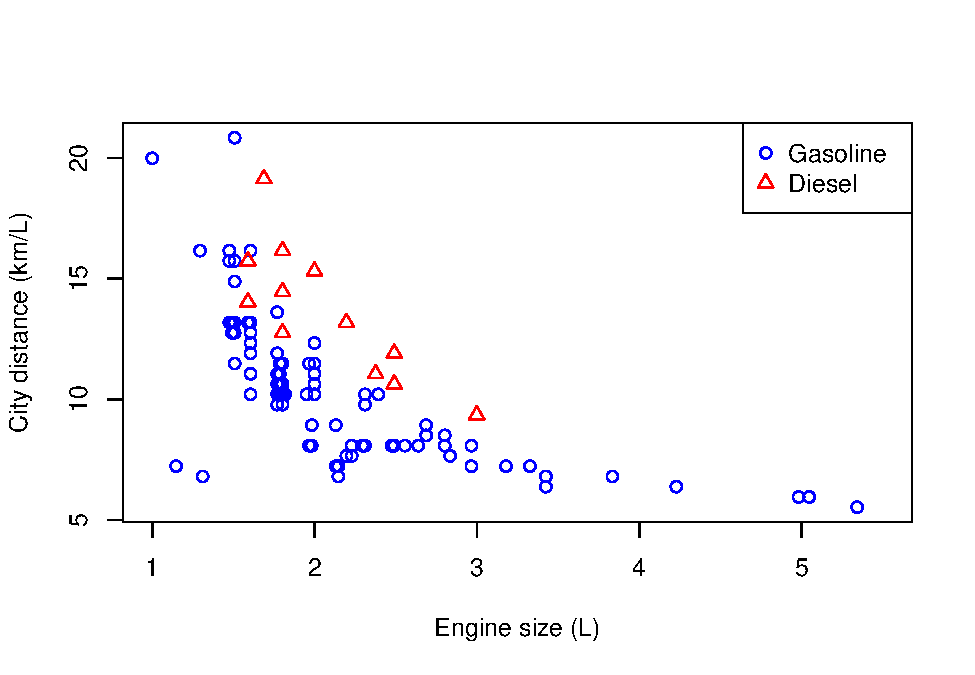
\includegraphics{oblig1_files/figure-latex/unnamed-chunk-2-1.pdf} A
linear model seems ok in the center of the bmi. But it is quite off in
the lower 1/4 and in the upper 1/4.We can see that the intercept and bmi
is strongly significant, indicating a strong correlation between bmi and
pdfm. The R-squared is siginificant, but not super high, so the model
can probably be improved. To see this clearly we plott indicitative
plotts on the fitness.

\begin{Shaded}
\begin{Highlighting}[]
\KeywordTok{plot}\NormalTok{(fit.simpleLinear)}
\end{Highlighting}
\end{Shaded}

\includegraphics{oblig1_files/figure-latex/unnamed-chunk-3-1.pdf}
\includegraphics{oblig1_files/figure-latex/unnamed-chunk-3-2.pdf}
\includegraphics{oblig1_files/figure-latex/unnamed-chunk-3-3.pdf}
\includegraphics{oblig1_files/figure-latex/unnamed-chunk-3-4.pdf}

\hypertarget{residuals-vs-fitted}{%
\paragraph{Residuals vs Fitted}\label{residuals-vs-fitted}}

Shows the Anscombe plot, wich would idealy present a eaven scattering
with no patterns in the points. In the plott we see a clear pattern, and
is indicating possiple violation of homoscedasicity. Meaning that
\epsiplon must be independent of the index.

\hypertarget{normal-q-q}{%
\paragraph{Normal Q-Q}\label{normal-q-q}}

This plot shows quantile-quantile plot. This plot shows the values of
the resiuals in increasing order. To see if the residuals folows a
normal distribution. For the assumption of normality to be valid we
would expect the values to folow the line in the plot. In the plot a
heavy tail and head can be observed. So the assumtion of normality is
not strong.

\hypertarget{scale-location}{%
\paragraph{Scale-Location}\label{scale-location}}

\hypertarget{residual-vs-leverage}{%
\paragraph{Residual vs Leverage}\label{residual-vs-leverage}}

\hypertarget{b}{%
\subsection{b}\label{b}}

We can see that we dont have any negative number, in such cases it is
often benefital to use a logarithmic transformation.

\begin{Shaded}
\begin{Highlighting}[]
\NormalTok{fit.log <-}\StringTok{ }\KeywordTok{lm}\NormalTok{(pbfm }\OperatorTok{~}\StringTok{ }\KeywordTok{log}\NormalTok{(bmi))}
\KeywordTok{print}\NormalTok{(}\KeywordTok{summary}\NormalTok{(fit.log))}
\end{Highlighting}
\end{Shaded}

\begin{verbatim}
## 
## Call:
## lm(formula = pbfm ~ log(bmi))
## 
## Residuals:
##      Min       1Q   Median       3Q      Max 
## -10.2548  -2.0453   0.1026   2.1238   8.6029 
## 
## Coefficients:
##             Estimate Std. Error t value Pr(>|t|)    
## (Intercept) -55.7327     2.3337  -23.88   <2e-16 ***
## log(bmi)     28.8031     0.6845   42.08   <2e-16 ***
## ---
## Signif. codes:  0 '***' 0.001 '**' 0.01 '*' 0.05 '.' 0.1 ' ' 1
## 
## Residual standard error: 3.125 on 325 degrees of freedom
## Multiple R-squared:  0.8449, Adjusted R-squared:  0.8444 
## F-statistic:  1771 on 1 and 325 DF,  p-value: < 2.2e-16
\end{verbatim}

\begin{Shaded}
\begin{Highlighting}[]
\NormalTok{beta =}\StringTok{ }\KeywordTok{coef}\NormalTok{(fit.log)}

\NormalTok{x =}\StringTok{ }\KeywordTok{log}\NormalTok{(}\KeywordTok{seq}\NormalTok{(}\KeywordTok{min}\NormalTok{(bmi), }\KeywordTok{max}\NormalTok{(bmi), }\DataTypeTok{length =} \DecValTok{200}\NormalTok{))}
\KeywordTok{plot}\NormalTok{(bmi, pbfm)}

\KeywordTok{lines}\NormalTok{(}\KeywordTok{exp}\NormalTok{(x),( beta[}\DecValTok{1}\NormalTok{] }\OperatorTok{+}\StringTok{ }\NormalTok{beta[}\DecValTok{2}\NormalTok{]}\OperatorTok{*}\StringTok{ }\NormalTok{x), }\DataTypeTok{col =} \DecValTok{2}\NormalTok{) }
\end{Highlighting}
\end{Shaded}

\includegraphics{oblig1_files/figure-latex/unnamed-chunk-4-1.pdf}

And to see how good the model is we plot some helping plots

\begin{Shaded}
\begin{Highlighting}[]
\KeywordTok{plot}\NormalTok{(fit.log)}
\end{Highlighting}
\end{Shaded}

\includegraphics{oblig1_files/figure-latex/unnamed-chunk-5-1.pdf}
\includegraphics{oblig1_files/figure-latex/unnamed-chunk-5-2.pdf}
\includegraphics{oblig1_files/figure-latex/unnamed-chunk-5-3.pdf}
\includegraphics{oblig1_files/figure-latex/unnamed-chunk-5-4.pdf}

It was also suggested to use a quadratic model.

\begin{Shaded}
\begin{Highlighting}[]
\NormalTok{fit.quad<-}\StringTok{ }\KeywordTok{lm}\NormalTok{(pbfm }\OperatorTok{~}\StringTok{ }\NormalTok{bmi }\OperatorTok{+}\StringTok{ }\KeywordTok{I}\NormalTok{(bmi}\OperatorTok{^}\DecValTok{2}\NormalTok{))}
\KeywordTok{print}\NormalTok{(}\KeywordTok{summary}\NormalTok{(fit.quad))}
\end{Highlighting}
\end{Shaded}

\begin{verbatim}
## 
## Call:
## lm(formula = pbfm ~ bmi + I(bmi^2))
## 
## Residuals:
##     Min      1Q  Median      3Q     Max 
## -9.3403 -1.9246  0.1433  1.8665  8.3780 
## 
## Coefficients:
##              Estimate Std. Error t value Pr(>|t|)    
## (Intercept) -11.17790    2.16977  -5.152 4.49e-07 ***
## bmi           2.53223    0.13229  19.142  < 2e-16 ***
## I(bmi^2)     -0.02448    0.00194 -12.617  < 2e-16 ***
## ---
## Signif. codes:  0 '***' 0.001 '**' 0.01 '*' 0.05 '.' 0.1 ' ' 1
## 
## Residual standard error: 3.036 on 324 degrees of freedom
## Multiple R-squared:  0.854,  Adjusted R-squared:  0.8531 
## F-statistic: 947.8 on 2 and 324 DF,  p-value: < 2.2e-16
\end{verbatim}

\begin{Shaded}
\begin{Highlighting}[]
\NormalTok{beta =}\StringTok{ }\KeywordTok{coef}\NormalTok{(fit.quad)}

\NormalTok{x =}\StringTok{ }\NormalTok{(}\KeywordTok{seq}\NormalTok{(}\KeywordTok{min}\NormalTok{(bmi), }\KeywordTok{max}\NormalTok{(bmi), }\DataTypeTok{length =} \DecValTok{200}\NormalTok{))}
\KeywordTok{plot}\NormalTok{(bmi, pbfm)}
\CommentTok{#points(bmi, pbfm)}
\KeywordTok{lines}\NormalTok{(x, beta[}\DecValTok{1}\NormalTok{] }\OperatorTok{+}\StringTok{ }\NormalTok{beta[}\DecValTok{2}\NormalTok{]}\OperatorTok{*}\NormalTok{x }\OperatorTok{+}\StringTok{ }\NormalTok{beta[}\DecValTok{3}\NormalTok{]}\OperatorTok{*}\NormalTok{x}\OperatorTok{^}\DecValTok{2}\NormalTok{, }\DataTypeTok{col=}\DecValTok{2}\NormalTok{)}
\end{Highlighting}
\end{Shaded}

\includegraphics{oblig1_files/figure-latex/unnamed-chunk-6-1.pdf} And
the acopening helping plots

\begin{Shaded}
\begin{Highlighting}[]
\KeywordTok{plot}\NormalTok{(fit.quad)}
\end{Highlighting}
\end{Shaded}

\includegraphics{oblig1_files/figure-latex/unnamed-chunk-7-1.pdf}
\includegraphics{oblig1_files/figure-latex/unnamed-chunk-7-2.pdf}
\includegraphics{oblig1_files/figure-latex/unnamed-chunk-7-3.pdf}
\includegraphics{oblig1_files/figure-latex/unnamed-chunk-7-4.pdf}

\hypertarget{c---leave-p-out-cross-validation-httpsen.wikipedia.orgwikicross-validation_statistics}{%
\subsection{\texorpdfstring{C - Leave-p-out cross-validation
(\url{https://en.wikipedia.org/wiki/Cross-validation_(statistics)})}{C - Leave-p-out cross-validation (https://en.wikipedia.org/wiki/Cross-validation\_(statistics))}}\label{c---leave-p-out-cross-validation-httpsen.wikipedia.orgwikicross-validation_statistics}}

\#max.p = 10 \#n = 4 \# n = len bmi \#shuffled = sample(1:length(bmi))
\#subset.size = length(bmi) \%/\% n \#indices\textless-matrix(list(),
nrow=n, ncol=1) \# indices{[}{[}1,1{]}{]} = shuffled{[}1:subset.size{]}
\# indices{[}{[}2,1{]}{]} = shuffled{[}subset.size +1:subset.size*2{]}
\# indices{[}{[}3,1{]}{]} = shuffled{[}(subset.size\emph{2 +
1):subset.size}3{]} \# indices{[}{[}4,1{]}{]} =
shuffled{[}(subset.size*3 + 1):length(bmi){]}

\#for(i in 0:n-1)\{ \# a = (subset.size\emph{i) + 1 \# b =
subset.size}(i+1) \# print(c(a,b)) \# indices{[}{[}i+1,1{]}{]} =
shuffled{[}a : b{]} \#\}

\#for (i in 1:max.p)\{ \# for(j in 0:n)\{ \# x = bmi{[}c(indices{[}{[}j
\%\% n{]}{]}, indices{[}{[}(j+1) \%\% n{]}{]}, indices{[}{[}(j+2) \%\%
n{]}{]}){]} \# y = pbfm{[}c(indices{[}{[}j \%\% n{]}{]},
indices{[}{[}(j+1) \%\% n{]}{]}, indices{[}{[}(j+2) \%\% n{]}{]}){]} \#
fit = lm(pbfm \textasciitilde{} poly(x, i), x = TRUE) \# x.test =
bmi{[}{]} \# \} \#\}

\hypertarget{problem-2}{%
\subsection{Problem 2}\label{problem-2}}

\begin{Shaded}
\begin{Highlighting}[]
\NormalTok{oral_ca <-}\StringTok{ }\KeywordTok{read.csv}\NormalTok{(}\StringTok{"oral_ca/oral_ca.csv"}\NormalTok{)}
\KeywordTok{attach}\NormalTok{(oral_ca)}
\KeywordTok{print}\NormalTok{(}\KeywordTok{summary}\NormalTok{(oral_ca))}
\end{Highlighting}
\end{Shaded}

\begin{verbatim}
##      drinks          ccstatus           cigs            age    
##  Min.   :  0.00   Min.   :0.0000   Min.   : 0.00   Min.   :21  
##  1st Qu.:  1.50   1st Qu.:0.0000   1st Qu.: 3.00   1st Qu.:48  
##  Median : 15.75   Median :0.0000   Median :20.00   Median :56  
##  Mean   : 31.40   Mean   :0.4887   Mean   :16.36   Mean   :56  
##  3rd Qu.: 48.00   3rd Qu.:1.0000   3rd Qu.:20.00   3rd Qu.:65  
##  Max.   :140.00   Max.   :1.0000   Max.   :60.00   Max.   :80  
##       sex            M_drinks            M_cigs       
##  Min.   :0.0000   Min.   :0.000000   Min.   :0.00000  
##  1st Qu.:0.0000   1st Qu.:0.000000   1st Qu.:0.00000  
##  Median :0.0000   Median :0.000000   Median :0.00000  
##  Mean   :0.2771   Mean   :0.005038   Mean   :0.01511  
##  3rd Qu.:1.0000   3rd Qu.:0.000000   3rd Qu.:0.00000  
##  Max.   :1.0000   Max.   :1.000000   Max.   :1.00000
\end{verbatim}

Aim of the study was to evaluate the risk of Oral cancer based on the
variables \textbf{drinks} (number og 1oz ethanol-equivalent drinks
consumed per week), \textbf{sex}, \textbf{age} and \textbf{cigs} (number
of cigaretts smoked per day).

\hypertarget{we-are-firs-interested-in-the-effect-of-smoking-alone}{%
\subsubsection{We are firs interested in the effect of smoking
alone}\label{we-are-firs-interested-in-the-effect-of-smoking-alone}}

\hypertarget{a-1}{%
\paragraph{(a)}\label{a-1}}

Q:

Dichotomize the variable cigs in two categories, smokers and not
smokers, and create a table with the observed frequencies for cases and
controls. In addition, provide the estimated probabilities (including
their standard errors) of experiencing an oral cancer (i.e., being a
case) for the two sub-populations.

A:

\begin{Shaded}
\begin{Highlighting}[]
\NormalTok{N =}\StringTok{ }\KeywordTok{length}\NormalTok{(oral_ca}\OperatorTok{$}\NormalTok{ccstatus)}
\NormalTok{smoker.nonSmoker =}\StringTok{ }\NormalTok{cigs }\OperatorTok{==}\StringTok{ }\DecValTok{0}
\NormalTok{smokers =}\StringTok{ }\KeywordTok{subset}\NormalTok{( oral_ca, oral_ca}\OperatorTok{$}\NormalTok{cigs }\OperatorTok{>}\StringTok{ }\DecValTok{0}\NormalTok{ )}\CommentTok{#smokers = oral_ca[ oral_ca$cigs > 0]}
\NormalTok{nonSmokers =}\StringTok{ }\KeywordTok{subset}\NormalTok{(oral_ca, oral_ca}\OperatorTok{$}\NormalTok{cigs }\OperatorTok{==}\StringTok{ }\DecValTok{0}\NormalTok{) }\CommentTok{#  nonSmokers = oral_ca[ oral_ca$cigs == 0 ]}
\NormalTok{number.of.cc =}\StringTok{ }\KeywordTok{nrow}\NormalTok{( }\KeywordTok{subset}\NormalTok{(oral_ca,oral_ca}\OperatorTok{$}\NormalTok{ccstatus }\OperatorTok{==}\StringTok{ }\DecValTok{1}\NormalTok{) )}
\NormalTok{number.of.cc.smokers =}\StringTok{ }\KeywordTok{nrow}\NormalTok{( }\KeywordTok{subset}\NormalTok{(oral_ca, oral_ca}\OperatorTok{$}\NormalTok{ccstatus }\OperatorTok{==}\StringTok{ }\DecValTok{1} \OperatorTok{&}\StringTok{ }\NormalTok{oral_ca}\OperatorTok{$}\NormalTok{cigs }\OperatorTok{>}\StringTok{ }\DecValTok{0}\NormalTok{) )}
\NormalTok{number.of.cc.nonSmokers =}\StringTok{ }\KeywordTok{nrow}\NormalTok{(}\KeywordTok{subset}\NormalTok{(oral_ca, oral_ca}\OperatorTok{$}\NormalTok{ccstatus }\OperatorTok{==}\StringTok{ }\DecValTok{1} \OperatorTok{&}\StringTok{ }\NormalTok{oral_ca}\OperatorTok{$}\NormalTok{cigs }\OperatorTok{==}\StringTok{ }\DecValTok{0}\NormalTok{) )}
\NormalTok{n.smoker =}\StringTok{ }\KeywordTok{nrow}\NormalTok{( }\KeywordTok{subset}\NormalTok{( oral_ca, oral_ca}\OperatorTok{$}\NormalTok{cigs }\OperatorTok{>}\StringTok{ }\DecValTok{0}\NormalTok{) )}
\NormalTok{n.nonSmoker =}\StringTok{ }\KeywordTok{nrow}\NormalTok{( }\KeywordTok{subset}\NormalTok{( oral_ca, oral_ca}\OperatorTok{$}\NormalTok{cigs }\OperatorTok{==}\StringTok{ }\DecValTok{0}\NormalTok{ ))}

\CommentTok{# Binomial - Mean}
\NormalTok{pi.common.hat =}\StringTok{ }\NormalTok{number.of.cc }\OperatorTok{/}\StringTok{ }\NormalTok{N }\CommentTok{# Number of ppl with cancer devided on ppl (people in the query )}
\NormalTok{pi.smoker.hat =}\StringTok{ }\NormalTok{number.of.cc.smokers }\OperatorTok{/}\StringTok{ }\NormalTok{n.smoker }\CommentTok{# Number of ppl with cancer and smokes, devided on number of ppl who smokes.}
\NormalTok{pi.nonSmoker.hat =}\StringTok{ }\NormalTok{number.of.cc.nonSmokers }\OperatorTok{/}\StringTok{ }\NormalTok{n.nonSmoker}\CommentTok{# Number of ppl with cancer and does not smoke, devided on number of ppl who does not soke.}

\CommentTok{# Binomial Vairance - Var(X) = n*p*(1-p)}
\NormalTok{se.pi.common =}\StringTok{ }\KeywordTok{sqrt}\NormalTok{(pi.common.hat }\OperatorTok{*}\StringTok{ }\NormalTok{(}\DecValTok{1} \OperatorTok{-}\StringTok{ }\NormalTok{pi.common.hat) }\OperatorTok{/}\StringTok{ }\NormalTok{N)}
\NormalTok{se.pi.smoker =}\StringTok{ }\KeywordTok{sqrt}\NormalTok{(pi.smoker.hat }\OperatorTok{*}\StringTok{ }\NormalTok{(}\DecValTok{1} \OperatorTok{-}\StringTok{ }\NormalTok{pi.nonSmoker.hat) }\OperatorTok{/}\NormalTok{n.smoker)}
\NormalTok{se.pi.nonSmoker =}\StringTok{ }\KeywordTok{sqrt}\NormalTok{(pi.nonSmoker.hat }\OperatorTok{*}\StringTok{ }\NormalTok{(}\DecValTok{1} \OperatorTok{-}\StringTok{ }\NormalTok{pi.nonSmoker.hat) }\OperatorTok{/}\NormalTok{n.nonSmoker)}

\NormalTok{cc.smoke.df  =}\StringTok{ }\KeywordTok{data.frame}\NormalTok{( }
  \DataTypeTok{pi =} \KeywordTok{c}\NormalTok{(pi.common.hat, pi.smoker.hat, pi.nonSmoker.hat), }
  \DataTypeTok{se =} \KeywordTok{c}\NormalTok{(se.pi.common, se.pi.smoker, se.pi.nonSmoker),}
  \DataTypeTok{row.names =} \KeywordTok{c}\NormalTok{(}\StringTok{"General"}\NormalTok{, }\StringTok{"Smoker"}\NormalTok{, }\StringTok{"NonSmoker"}\NormalTok{)}
\NormalTok{  )}
\end{Highlighting}
\end{Shaded}

\hypertarget{b-1}{%
\paragraph{(b)}\label{b-1}}

Q:

Test the hypothesis that the two probabilities are equal and comment on
the result.

A:

Hypothesis: H0: probSmokers == probNonSmokers against H1: probSmokers !=
probNonSmokers. Computing the p-value

\begin{Shaded}
\begin{Highlighting}[]
\CommentTok{# compute the likelihood ratio statistics test}
\NormalTok{llik_pi.smoker.hat_pi.nonSmoker.hat =}\StringTok{ }\KeywordTok{sum}\NormalTok{(}\KeywordTok{dbinom}\NormalTok{(smoker.nonSmoker[ smoker.nonSmoker }\OperatorTok{==}\StringTok{ }\OtherTok{TRUE}\NormalTok{], }\DecValTok{1}\NormalTok{, pi.smoker.hat, }\DataTypeTok{log =} \OtherTok{TRUE}\NormalTok{)) }\OperatorTok{+}\StringTok{ }
\StringTok{                                      }\KeywordTok{sum}\NormalTok{(}\KeywordTok{dbinom}\NormalTok{(smoker.nonSmoker[ smoker.nonSmoker }\OperatorTok{==}\StringTok{ }\OtherTok{FALSE}\NormalTok{], }\DecValTok{1}\NormalTok{, pi.nonSmoker.hat, }\DataTypeTok{log =} \OtherTok{TRUE}\NormalTok{))}
\NormalTok{llik_pi.common.hat =}\StringTok{ }\KeywordTok{sum}\NormalTok{(}\KeywordTok{dbinom}\NormalTok{(smoker.nonSmoker, }\DecValTok{1}\NormalTok{, pi.common.hat, }\DataTypeTok{log=}\OtherTok{TRUE}\NormalTok{))}

\NormalTok{w =}\StringTok{ }\DecValTok{2} \OperatorTok{*}\StringTok{ }\NormalTok{(llik_pi.smoker.hat_pi.nonSmoker.hat }\OperatorTok{-}\StringTok{ }\NormalTok{llik_pi.common.hat)}
\NormalTok{p.val =}\StringTok{ }\DecValTok{1} \OperatorTok{-}\StringTok{ }\KeywordTok{pchisq}\NormalTok{(w, }\DataTypeTok{df =} \DecValTok{1}\NormalTok{)}
\end{Highlighting}
\end{Shaded}

We can se that the p-val is zero, so we can drop H0.

\hypertarget{c}{%
\paragraph{(c)}\label{c}}

Q:

Fit a linear logistic model using the dichotomized variable as
explanatory variable and comment on the result: does being a smoker
increase or decrease the risk of experiencing oral cancer? How much, in
terms of log-odds?

A:

\begin{Shaded}
\begin{Highlighting}[]
\NormalTok{y =}\StringTok{ }\NormalTok{oral_ca}\OperatorTok{$}\NormalTok{ccstatus }\OperatorTok{==}\StringTok{ }\DecValTok{1}
\NormalTok{x =}\StringTok{ }\NormalTok{oral_ca}\OperatorTok{$}\NormalTok{cigs }\OperatorTok{>}\StringTok{ }\DecValTok{0}

\NormalTok{mod =}\StringTok{ }\KeywordTok{glm}\NormalTok{(y }\OperatorTok{~}\StringTok{ }\NormalTok{x, }\DataTypeTok{family =} \StringTok{'binomial'}\NormalTok{)}
\KeywordTok{print}\NormalTok{(}\KeywordTok{summary}\NormalTok{(mod))}
\end{Highlighting}
\end{Shaded}

\begin{verbatim}
## 
## Call:
## glm(formula = y ~ x, family = "binomial")
## 
## Deviance Residuals: 
##    Min      1Q  Median      3Q     Max  
## -1.285  -1.285  -0.744   1.073   1.685  
## 
## Coefficients:
##             Estimate Std. Error z value Pr(>|z|)    
## (Intercept)  -1.1431     0.2448  -4.669 3.03e-06 ***
## xTRUE         1.3927     0.2706   5.147 2.65e-07 ***
## ---
## Signif. codes:  0 '***' 0.001 '**' 0.01 '*' 0.05 '.' 0.1 ' ' 1
## 
## (Dispersion parameter for binomial family taken to be 1)
## 
##     Null deviance: 550.15  on 396  degrees of freedom
## Residual deviance: 520.14  on 395  degrees of freedom
## AIC: 524.14
## 
## Number of Fisher Scoring iterations: 4
\end{verbatim}

\begin{Shaded}
\begin{Highlighting}[]
\NormalTok{beta =}\StringTok{ }\NormalTok{mod}\OperatorTok{$}\NormalTok{coefficients}
\KeywordTok{print}\NormalTok{(beta)}
\end{Highlighting}
\end{Shaded}

\begin{verbatim}
## (Intercept)       xTRUE 
##   -1.143064    1.392719
\end{verbatim}

\begin{Shaded}
\begin{Highlighting}[]
\NormalTok{pi.nonSmoker =}\StringTok{ }\KeywordTok{exp}\NormalTok{(beta[}\DecValTok{1}\NormalTok{]) }\OperatorTok{/}\StringTok{ }\NormalTok{(}\DecValTok{1} \OperatorTok{+}\StringTok{ }\KeywordTok{exp}\NormalTok{(beta[}\DecValTok{1}\NormalTok{]))}
\NormalTok{pi.smoker =}\StringTok{ }\KeywordTok{exp}\NormalTok{(beta[}\DecValTok{1}\NormalTok{] }\OperatorTok{+}\StringTok{ }\NormalTok{beta[}\DecValTok{2}\NormalTok{]) }\OperatorTok{/}\StringTok{ }\NormalTok{(}\DecValTok{1} \OperatorTok{+}\StringTok{ }\KeywordTok{exp}\NormalTok{(beta[}\DecValTok{1}\NormalTok{] }\OperatorTok{+}\StringTok{ }\NormalTok{beta[}\DecValTok{2}\NormalTok{]))}

\CommentTok{#odds}
\NormalTok{odds.nonSmoker =}\StringTok{ }\NormalTok{pi.nonSmoker.hat }\OperatorTok{/}\StringTok{ }\NormalTok{(}\DecValTok{1} \OperatorTok{-}\StringTok{ }\NormalTok{pi.nonSmoker.hat)}
\NormalTok{odds.smoker =}\StringTok{ }\NormalTok{pi.smoker.hat }\OperatorTok{/}\StringTok{ }\NormalTok{(}\DecValTok{1} \OperatorTok{-}\StringTok{ }\NormalTok{pi.smoker.hat)}
\CommentTok{#log odds ratio}
\NormalTok{log.odds.ratio =}\StringTok{ }\NormalTok{(odds.smoker }\OperatorTok{/}\StringTok{ }\NormalTok{odds.nonSmoker)}

\NormalTok{log.odds.ratio}
\end{Highlighting}
\end{Shaded}

\begin{verbatim}
## [1] 4.02578
\end{verbatim}

We see that the odds of cc for a smoker against a non somoker is aprox
4, aka. 4 to 1.

\hypertarget{d}{%
\paragraph{(d)}\label{d}}

Q:

Repeat the analysis of point (c) by considering, now, the number of
cigarettes as a continuous variable. Comment on the result: What does
the regression coefficient for this variable mean now? Why does the
value of the intercept change with respect to point (c), although they
are both related to the odds for non-smokers?

A:

\begin{Shaded}
\begin{Highlighting}[]
\NormalTok{x =}\StringTok{ }\NormalTok{cigs}
\NormalTok{y =}\StringTok{ }\NormalTok{ccstatus}
\NormalTok{mod.continuous =}\StringTok{ }\KeywordTok{glm}\NormalTok{(y }\OperatorTok{~}\StringTok{ }\NormalTok{x, }\DataTypeTok{family =} \StringTok{'binomial'}\NormalTok{)}
\KeywordTok{print}\NormalTok{(}\KeywordTok{summary}\NormalTok{(mod.continuous))}
\end{Highlighting}
\end{Shaded}

\begin{verbatim}
## 
## Call:
## glm(formula = y ~ x, family = "binomial")
## 
## Deviance Residuals: 
##     Min       1Q   Median       3Q      Max  
## -2.1923  -1.0237  -0.8228   1.1088   1.5796  
## 
## Coefficients:
##              Estimate Std. Error z value Pr(>|z|)    
## (Intercept) -0.909057   0.171766  -5.292 1.21e-07 ***
## x            0.053624   0.008614   6.225 4.81e-10 ***
## ---
## Signif. codes:  0 '***' 0.001 '**' 0.01 '*' 0.05 '.' 0.1 ' ' 1
## 
## (Dispersion parameter for binomial family taken to be 1)
## 
##     Null deviance: 550.15  on 396  degrees of freedom
## Residual deviance: 504.39  on 395  degrees of freedom
## AIC: 508.39
## 
## Number of Fisher Scoring iterations: 4
\end{verbatim}

The regression coefficient now tells us the increase in odds of cancer
per cigarets smoked per day. The intercept is changed since smoking one
sigaret per day is closer to zero than smoking 20. In the non continius
model the biggest smoker and the rest is given the same odds.

\hypertarget{consider-now-the-other-three-variables-drinks-sex-and-age-as-well}{%
\subsubsection{Consider now the other three variables (drinks, sex and
age) as
well:}\label{consider-now-the-other-three-variables-drinks-sex-and-age-as-well}}

\hypertarget{e}{%
\paragraph{(e)}\label{e}}

Q:

Fit a linear logistic model including all the explanatory variables and
report the result. What is the increase in terms of log-odds for an
increasing number of cigarettes per day smoked estimated by this model?
Why did it change from the one obtained in model fitted in point (c)?

\begin{Shaded}
\begin{Highlighting}[]
\NormalTok{mod.all =}\StringTok{ }\KeywordTok{glm}\NormalTok{(y }\OperatorTok{~}\StringTok{  }\NormalTok{oral_ca}\OperatorTok{$}\NormalTok{drinks }\OperatorTok{+}\StringTok{ }\NormalTok{oral_ca}\OperatorTok{$}\NormalTok{cigs }\OperatorTok{+}\StringTok{ }\NormalTok{oral_ca}\OperatorTok{$}\NormalTok{age }\OperatorTok{+}\StringTok{ }\NormalTok{oral_ca}\OperatorTok{$}\NormalTok{sex, }\DataTypeTok{family =} \StringTok{'binomial'}\NormalTok{)}
\KeywordTok{print}\NormalTok{(}\KeywordTok{summary}\NormalTok{(mod.all))}
\end{Highlighting}
\end{Shaded}

\begin{verbatim}
## 
## Call:
## glm(formula = y ~ oral_ca$drinks + oral_ca$cigs + oral_ca$age + 
##     oral_ca$sex, family = "binomial")
## 
## Deviance Residuals: 
##     Min       1Q   Median       3Q      Max  
## -2.7185  -0.8589  -0.5832   0.9644   1.9776  
## 
## Coefficients:
##                 Estimate Std. Error z value Pr(>|z|)    
## (Intercept)    -1.966071   0.620756  -3.167  0.00154 ** 
## oral_ca$drinks  0.029623   0.004643   6.380 1.77e-10 ***
## oral_ca$cigs    0.035480   0.009571   3.707  0.00021 ***
## oral_ca$age     0.006529   0.009960   0.656  0.51213    
## oral_ca$sex     0.594499   0.272752   2.180  0.02928 *  
## ---
## Signif. codes:  0 '***' 0.001 '**' 0.01 '*' 0.05 '.' 0.1 ' ' 1
## 
## (Dispersion parameter for binomial family taken to be 1)
## 
##     Null deviance: 550.15  on 396  degrees of freedom
## Residual deviance: 443.84  on 392  degrees of freedom
## AIC: 453.84
## 
## Number of Fisher Scoring iterations: 5
\end{verbatim}

The increase in terms of log-odds for an increasing number of cigaretts
par day by this model is 0.035, wich is a little lower than in the
prewius model. This can be because of some of the affects of other
facors was tried explained by one facotr. Now we have other factors to
explain this change. Wich will change the value.

\hypertarget{e-1}{%
\paragraph{(e)}\label{e-1}}

\begin{Shaded}
\begin{Highlighting}[]
\NormalTok{mod.without.Age =}\StringTok{ }\KeywordTok{glm}\NormalTok{(y }\OperatorTok{~}\StringTok{  }\NormalTok{oral_ca}\OperatorTok{$}\NormalTok{drinks }\OperatorTok{+}\StringTok{ }\NormalTok{oral_ca}\OperatorTok{$}\NormalTok{cigs }\OperatorTok{+}\StringTok{ }\NormalTok{oral_ca}\OperatorTok{$}\NormalTok{sex, }\DataTypeTok{family =} \StringTok{'binomial'}\NormalTok{)}
\KeywordTok{print}\NormalTok{(}\KeywordTok{summary}\NormalTok{(mod.without.Age))}
\end{Highlighting}
\end{Shaded}

\begin{verbatim}
## 
## Call:
## glm(formula = y ~ oral_ca$drinks + oral_ca$cigs + oral_ca$sex, 
##     family = "binomial")
## 
## Deviance Residuals: 
##     Min       1Q   Median       3Q      Max  
## -2.6943  -0.8596  -0.6084   0.9607   1.8857  
## 
## Coefficients:
##                 Estimate Std. Error z value Pr(>|z|)    
## (Intercept)    -1.592919   0.238787  -6.671 2.54e-11 ***
## oral_ca$drinks  0.029498   0.004638   6.360 2.01e-10 ***
## oral_ca$cigs    0.035536   0.009565   3.715 0.000203 ***
## oral_ca$sex     0.582183   0.271756   2.142 0.032169 *  
## ---
## Signif. codes:  0 '***' 0.001 '**' 0.01 '*' 0.05 '.' 0.1 ' ' 1
## 
## (Dispersion parameter for binomial family taken to be 1)
## 
##     Null deviance: 550.15  on 396  degrees of freedom
## Residual deviance: 444.27  on 393  degrees of freedom
## AIC: 452.27
## 
## Number of Fisher Scoring iterations: 5
\end{verbatim}

\begin{Shaded}
\begin{Highlighting}[]
\KeywordTok{plot}\NormalTok{(mod.without.Age)}
\end{Highlighting}
\end{Shaded}

\includegraphics{oblig1_files/figure-latex/unnamed-chunk-14-1.pdf}
\includegraphics{oblig1_files/figure-latex/unnamed-chunk-14-2.pdf}
\includegraphics{oblig1_files/figure-latex/unnamed-chunk-14-3.pdf}
\includegraphics{oblig1_files/figure-latex/unnamed-chunk-14-4.pdf}

Since the explanatory variable age has a large p-value can we not say it
gives significant value to the model. So it does not seem like there is
a difference in age. Lookin at the deviance the age variable did noting
significant for the model ether. So i would choose the one with less
explanatory variables, aka the one without Age

\hypertarget{g}{%
\paragraph{(g)}\label{g}}

Q:

Use a polynomial of degree 2 to model the effect of drinks. Does it
improve the model?

A:

\begin{Shaded}
\begin{Highlighting}[]
\NormalTok{mod.quad.drinks =}\StringTok{ }\KeywordTok{glm}\NormalTok{(y }\OperatorTok{~}\StringTok{  }\NormalTok{oral_ca}\OperatorTok{$}\NormalTok{drinks }\OperatorTok{+}\StringTok{ }\KeywordTok{I}\NormalTok{(oral_ca}\OperatorTok{$}\NormalTok{drinks}\OperatorTok{^}\DecValTok{2}\NormalTok{) }\OperatorTok{+}\StringTok{ }\NormalTok{oral_ca}\OperatorTok{$}\NormalTok{cigs }\OperatorTok{+}\StringTok{ }\NormalTok{oral_ca}\OperatorTok{$}\NormalTok{sex, }\DataTypeTok{family =} \StringTok{'binomial'}\NormalTok{)}
\KeywordTok{print}\NormalTok{(}\KeywordTok{summary}\NormalTok{(mod.quad.drinks))}
\end{Highlighting}
\end{Shaded}

\begin{verbatim}
## 
## Call:
## glm(formula = y ~ oral_ca$drinks + I(oral_ca$drinks^2) + oral_ca$cigs + 
##     oral_ca$sex, family = "binomial")
## 
## Deviance Residuals: 
##     Min       1Q   Median       3Q      Max  
## -2.2192  -0.8379  -0.5405   0.8756   1.9980  
## 
## Coefficients:
##                       Estimate Std. Error z value Pr(>|z|)    
## (Intercept)         -1.850e+00  2.667e-01  -6.936 4.03e-12 ***
## oral_ca$drinks       5.362e-02  1.052e-02   5.099 3.42e-07 ***
## I(oral_ca$drinks^2) -2.295e-04  8.419e-05  -2.726 0.006405 ** 
## oral_ca$cigs         3.301e-02  9.642e-03   3.424 0.000618 ***
## oral_ca$sex          7.256e-01  2.854e-01   2.542 0.011007 *  
## ---
## Signif. codes:  0 '***' 0.001 '**' 0.01 '*' 0.05 '.' 0.1 ' ' 1
## 
## (Dispersion parameter for binomial family taken to be 1)
## 
##     Null deviance: 550.15  on 396  degrees of freedom
## Residual deviance: 437.62  on 392  degrees of freedom
## AIC: 447.62
## 
## Number of Fisher Scoring iterations: 4
\end{verbatim}

\begin{Shaded}
\begin{Highlighting}[]
\KeywordTok{plot}\NormalTok{(mod.quad.drinks)}
\end{Highlighting}
\end{Shaded}

\includegraphics{oblig1_files/figure-latex/unnamed-chunk-15-1.pdf}
\includegraphics{oblig1_files/figure-latex/unnamed-chunk-15-2.pdf}
\includegraphics{oblig1_files/figure-latex/unnamed-chunk-15-3.pdf}
\includegraphics{oblig1_files/figure-latex/unnamed-chunk-15-4.pdf}

The change to a quadratic polynomial for the drinks varibale did not
seem to change much, it is a small variable comaring to the other once,
but have a sigificant p-value. The p-value can be caused by the hig
similarity between drinks and drinks\^{}2, this theory is strengthen by
the increase in the p-value of drinks.

\hypertarget{h}{%
\paragraph{(h)}\label{h}}

Q:

What about doing that for cigs instead of drinks? What is the effect on
the model?

A:

\begin{Shaded}
\begin{Highlighting}[]
\NormalTok{mod.quad.smokes =}\StringTok{ }\KeywordTok{glm}\NormalTok{(y }\OperatorTok{~}\StringTok{  }\NormalTok{oral_ca}\OperatorTok{$}\NormalTok{drinks }\OperatorTok{+}\StringTok{ }\NormalTok{oral_ca}\OperatorTok{$}\NormalTok{cigs}\OperatorTok{+}\StringTok{ }\KeywordTok{I}\NormalTok{(oral_ca}\OperatorTok{$}\NormalTok{cigs}\OperatorTok{^}\DecValTok{2}\NormalTok{) }\OperatorTok{+}\StringTok{ }\NormalTok{oral_ca}\OperatorTok{$}\NormalTok{sex, }\DataTypeTok{family =} \StringTok{'binomial'}\NormalTok{)}
\KeywordTok{print}\NormalTok{(}\KeywordTok{summary}\NormalTok{(mod.quad.smokes))}
\end{Highlighting}
\end{Shaded}

\begin{verbatim}
## 
## Call:
## glm(formula = y ~ oral_ca$drinks + oral_ca$cigs + I(oral_ca$cigs^2) + 
##     oral_ca$sex, family = "binomial")
## 
## Deviance Residuals: 
##     Min       1Q   Median       3Q      Max  
## -2.6870  -0.8764  -0.5808   0.9695   1.9303  
## 
## Coefficients:
##                     Estimate Std. Error z value Pr(>|z|)    
## (Intercept)       -1.6943120  0.2697349  -6.281 3.36e-10 ***
## oral_ca$drinks     0.0289791  0.0046347   6.253 4.04e-10 ***
## oral_ca$cigs       0.0541177  0.0238775   2.266   0.0234 *  
## I(oral_ca$cigs^2) -0.0004485  0.0005225  -0.858   0.3907    
## oral_ca$sex        0.6019008  0.2742844   2.194   0.0282 *  
## ---
## Signif. codes:  0 '***' 0.001 '**' 0.01 '*' 0.05 '.' 0.1 ' ' 1
## 
## (Dispersion parameter for binomial family taken to be 1)
## 
##     Null deviance: 550.15  on 396  degrees of freedom
## Residual deviance: 443.55  on 392  degrees of freedom
## AIC: 453.55
## 
## Number of Fisher Scoring iterations: 5
\end{verbatim}

\begin{Shaded}
\begin{Highlighting}[]
\KeywordTok{plot}\NormalTok{(mod.quad.smokes)}
\end{Highlighting}
\end{Shaded}

\includegraphics{oblig1_files/figure-latex/unnamed-chunk-16-1.pdf}
\includegraphics{oblig1_files/figure-latex/unnamed-chunk-16-2.pdf}
\includegraphics{oblig1_files/figure-latex/unnamed-chunk-16-3.pdf}
\includegraphics{oblig1_files/figure-latex/unnamed-chunk-16-4.pdf}

Adding cigs\^{}2 as a variable also did not change the model much. Here
the cigs\^{}2 variable eaven has a high p-value, showing the
insignificance of the variable.

\hypertarget{i}{%
\paragraph{(i)}\label{i}}

Adding the quadratic variables did not seem to give the biggest effect.
It seems to make the none suared variable (cigs, drinks) less
significant with a compareble degree the quadratic values give to the
model. So they might be better but not significantly. No significant
difference in the residuals ether.

\hypertarget{j}{%
\paragraph{(j)}\label{j}}

If the model fit a quareatic scale, that means that two drinks is more
then twice as bad than one drink. It does not necessarily make it worse
to drink 10 units, if the model fits with linear or quadratic wariables,
it will just change the coefficients. A way to explain this is with the
functions

f(x = 10) = beta * x = a, and f(x = 10) = beta1 * x + beta2 * x\^{}2 =
a.

The point of the function is to show that if you drink 10 drinks and the
relation is linear can be the same as drinking 10 drinks in a quadradic
model. This is correct in all polynomials.

\hypertarget{k}{%
\paragraph{(k)}\label{k}}

\ldots{}

\hypertarget{komment-1}{%
\subsection{Komment}\label{komment-1}}

\end{document}
